\documentclass[a4paper, 11pt]{article}

\usepackage{geometry}
\usepackage{natbib}
\bibpunct[:]{(}{)}{,}{a}{}{;}

%--------------------
%\usepackage{gb4e}
%\noautomath

\usepackage{amsmath}
\usepackage{amsfonts}
\usepackage{amsthm}
\usepackage{amssymb}
\usepackage{mathrsfs}
\usepackage{nicefrac}
%\usepackage{stmaryrd}
%\usepackage{multicol}
\usepackage{graphicx}
\usepackage{color}
\usepackage{booktabs}
\usepackage{pgfplots}
\usepackage{subcaption}
\pgfplotsset{compat=1.3}
\usetikzlibrary{pgfplots.groupplots,decorations.markings}


%\newcommand{\mvalueof}[1]{\llbracket#1\rrbracket}
\newcommand{\citeposs}[2][]{\citeauthor{#2}'s (\citeyear[#1]{#2})}
\newcommand{\tuple}[1]{\ensuremath{\left\langle #1 \right\rangle}} 

\newcommand{\hl}[1]{\textcolor[rgb]{.8,.33,.0}{#1}}% prints in orange
%\newcommand{\argmax}[1]{\underset{#1}{\operatorname{arg}\,\operatorname{max}}\;}
%\newcommand{\argmin}[1]{\underset{#1}{\operatorname{arg}\,\operatorname{min}}\;}
%\newcommand{\sbna}{\exists\lnot\forall}

\definecolor{Red}{RGB}{178,34,34}
\newcommand{\mf}[1]{\textcolor{Red}{[MF: #1]}} 
\newcommand{\tb}[1]{\textcolor[rgb]{.8,.33,.0}{[TB: #1]}}% prints in orange

\usepackage{blkarray}
\usepackage{xspace}

\usepackage{tgtermes}
\renewcommand{\baselinestretch}{1.2}

%%% MF's commands
\newcommand{\set}[1]{\left\{#1\right\}}
\newcommand{\card}[1]{\left \lvert \, #1 \, \right\rvert}
\newcommand{\abs}[1]{\lvert #1 \rvert}
\newcommand{\States}{\ensuremath{S}\xspace}		% Set of States
\newcommand{\state}{\ensuremath{s}\xspace}		% single states
\newcommand{\mystate}[1]{\ensuremath{\state_{\text{#1}}}\xspace} %meaningful states
\newcommand{\mylang}[1]{\ensuremath{L_{\text{#1}}}\xspace} %meaningful states
\newcommand{\Messgs}{\ensuremath{M}\xspace}		% Set of Messages
\newcommand{\messg}{\ensuremath{m}\xspace}		% single messages
\newcommand{\mymessg}[1]{\ensuremath{\messg_{\text{#1}}}\xspace} %meaningful messages
\newcommand{\ssome}{\mystate{\ensuremath{\exists\neg\forall}}}
\newcommand{\sall}{\mystate{\ensuremath{\forall}}}
\newcommand{\snone}{\mystate{\ensuremath{\emptyset}}}
\newcommand{\msome}{\mymessg{some}}
\newcommand{\mall}{\mymessg{all}}
\newcommand{\mnone}{\mymessg{none}}
\newcommand{\Lall}{\mylang{all}}
\newcommand{\Lbound}{\mylang{bound}}
\newcommand{\Llack}{\mylang{lack}}
\newcommand{\asome}{\myact{\ensuremath{\exists\neg\forall}}}
\newcommand{\aall}{\myact{\ensuremath{\forall}}}

\definecolor{mygray}{cmyk}{0.35,0.35,0.35,0.35}
\newcommand{\mygray}[1]{{\textcolor{mygray}{#1}}}
%%% 


%--------------------
%
%\usepackage{setspace}
%\onehalfspacing
%
%-------------------


\title{Tracing the cultural evolution of meaning at the semantics-pragmatics interface}

\author{%\bf NAME1 and NAME2\\
    ( -- draft \today --- )
}


\date{}

\begin{document}

  %% for arrow head placement
  \tikzset{->-/.style={decoration={
  markings,
  mark=at position #1 with {\arrow{>}}},postaction={decorate}}}
  %%% 

\maketitle

\begin{abstract}
  According to standard linguistic theory, the meaning of an utterance is the product of
  conventional semantic meaning and general pragmatic rules on language use. To investigate how
  cultural evolution of language plays out under this picture of the semantics-pragmatics
  interface, we present a game theoretic model of the competition between types of language
  users, each endowed with her selection of lexical concepts and her own pragmatic dispositions
  to act on them. Our model traces two evolutionary forces and their interaction: (i)
  fitness-based pressure towards communicative efficiency and (ii) potential learning biases
  during the transfer of linguistic knowledge. We illustrate the model based on a case study on
  scalar implicatures. In this case study learning biases that favor simple semantic
  representations can boost the evolution of more sophisticated pragmatic reasoning types and
  so prevent the lexicalization of scalar implicatures.
\end{abstract}

\section{Introduction}\label{sec:introduction}
What is conveyed usually goes beyond what is said. A request for a blanket can be politely
veiled by uttering ``I'm cold;'' temporal succession of events can be communicated by the order
in which conjuncts appear as in ``I traveled to Paris and got married;'' an invitation can be
declined by saying ``I have to work.'' An influential explanation of the relation between the
literal meaning of expressions and what they may convey in context is due to
\citet{grice:1975}, who characterizes pragmatic use and interpretation as a process of mutual
reasoning about rational language use. For instance, under the assumption that the speaker is
cooperative and relevant, ``I have to work'' may be interpreted as providing a reason why the
speaker will not be able to accept an invitation, going beyond its literal meaning. Some of
these enrichments are rather \emph{ad hoc}. Others show striking regularities, such as the use
of ability questions for polite requests (``Could you please \dots?''), or certain enrichments
of lexical meanings such as \emph{and} to convey \emph{and then}.

A particularly productive and well studied class of systematic pragmatic enrichments are scalar
implicatures
\citep{horn:1984,Hirschberg1985:A-Theory-of-Sca,LevinsonPragmatics1983,Geurts2010:Quantity-Implic}. Usually,
the utterance of a sentence like ``I own some of Johnny Cash's albums'' will be taken to mean
that the speaker does not own all of them. This is because, if the speaker owned them all, she
could have used the word \emph{all} instead of \emph{some} in his utterance, thereby making a
more informative statement. Scalar implicatures, especially the inference from \emph{some} to
\emph{some but not all}, have been studied extensively, both theoretically
\citep[e.g.,][]{Sauerland2004:Scalar-Implicat,ChierchiaFox2008:The-Grammatical,Rooyvan-RooijJagerde-Jager2012:Explaining-Quan}
as well as experimentally
\citep[e.g.,][]{BottNoveck2004:Some-Utterances,huang+snedeker:2009,GrodnerKlein2010:Some-and-Possib,GoodmanStuhlmuller2013:Knowledge-and-I,DegenTanenhaus2012:Processing-Scal}. While
there is much dispute in this domain about many details, a position endorsed by a clear
majority is that a scalar item like \emph{some} is underspecified to mean \emph{some and maybe
  all} and that the enrichment to \emph{some but not all} is part of some regular process with
roots in pragmatics.

If this majority view is correct, the question arises how such a division of labor between
semantics and pragmatics could have evolved and why it would be so pervasive across natural
languages. Models of language evolution abound. There are simulation-based models studying the
evolution of language in populations of communicating agents
\citep{Hurford1989:Biological-Evol,Steels1995:A-Self-Organizi,LenaertsJansen2005:The-Evolutionar,SteelsBelpaeme2005:Coordinating-Pe,BaronchelliPuglisi2008:Cultural-route-,steels:2011,SpikeStadler2016:Minimal-Require}
and there are mathematical models of language evolution, mostly coming from game theory
\citep{lewis:1969,Warneryd1993:Cheap-Talk-Coor,BlumeKim1993:Evolutionary-St,nowak+krakauer:1999,Huttegger2007:Evolution-and-t,Skyrms2010:Signals}. Much
of this work has focused on explaining basic properties such as compositionality and
combinatoriality
\citep[e.g.,][]{Batali1998:Computational-S,nowak+krakauer:1999,nowak+etal:2000,KirbyHurford2002:The-Emergence-o,kirby:2002,SmithKirby2003:Iterated-Learni,Gong2007:Language-Evolut,kirby+etal:2015,verhoef+etal:2014,Franke2015:Proto-Syntax},
but little attention has been paid to the interaction between conventional meaning and
pragmatic use. What is more, many mathematical models explain evolved meaning as a regularity
in the overt behavior of agents. In contrast, we will here look at language users with a richer
cognitive make-up and their dispositions to act.


Towards this end, we spell out a model of the co-evolution of conventional meaning and
pragmatic reasoning types. The objects of replication and selection are pairs of lexical
meanings and general types of pragmatic behavior, which we represent using probabilistic models
of pragmatic language use
\citep{frank+goodman:2012,FrankeJager2015:Probabilistic-p,GoodmanFrank2016:Pragmatic-Langu}. Replication
and selection are described by the \emph{replicator mutator dynamic}, a general and established
model of evolutionary change in large and homogeneous populations
\citep{Hofbauer1985:The-Selection-M,nowak+etal:2000,NowakKomarova2001:Evolution-of-Un,hofbauer+sigmund:2003,Nowak2006:Evolutionary-Dy}. The
approach allows us to study the interaction between (i) evolutionary pressure towards
communicative efficiency and (ii) possible infidelity in the transmission of linguistic
knowledge, caused by factors such as inductive learning biases and sparse learning
data. Considering transmission of linguistic knowledge is important because neither semantic
meanings nor pragmatic usage patterns are directly observable. Instead, language learners have
to infer these unobservables from the observable behavior in which they result. We formalize
this process as a form of Bayesian inference. Our approach thereby contains a well-understood
model of iterated Bayesian learning \citep{griffiths+kalish:2007} as a special case, but
combines it with functional selection, here formalized as the most versatile dynamic from
evolutionary game theory; the replicator dynamic
\citep{TaylorJonker1978:Evolutionary-St}. Section~\ref{sec:model} introduces this model.

Section~\ref{sec:si-case-study} applies this model to a case study on scalar implicatures. We
discuss a setting in which the majority view of underspecified lexical meanings and pragmatic
enrichments emerges if selection and transmission infidelity are combined. In particular, we
show that inductive learning biases of Bayesian learners that favor simpler lexical meanings
can prevent the lexicalization of scalar inferences and lead to the emergence of Gricean-like
pragmatic reasoning types. Results of this case study are critically assessed in the light of
the assumptions that feed our model in Section~\ref{sec:discussion}.

% We see the main contribution of this work as conceptual and technical, not as a definite answer
% to the question why scalar implicatures emerge. It rather demonstrates how current
% probabilistic cognitive modeling of language use and evolutionary modeling can be fruitfully
% combined to study the co-evolution of semantics and pragmatics side-by-side. Reversely, the
% approach taken here may be seen as a first step towards giving an evolutionary rationale for
% empirically successful probabilistic models of language use that embrace the majority view of
% the division of labor between semantics and pragmatics. Section~\ref{sec:discussion} elaborates
% on these points.

\section{A model of co-evolving lexical concepts and pragmatic behavior}
\label{sec:model}

\subsection{Expressivity and learnability}

The emergence and change of linguistic structure is influenced by many intertwined
factors. These range from biological and socio-ecological to cultural ones \citep{benz+etal:2005b,steels:2011,tamariz+kirby:2016}. Social and ecological pressures determine communicative needs, while
biology determines the architecture that enables and constrains the means by which they can be
fulfilled. In the following, our focus lies on cultural aspects, wherein processes of
linguistic change are viewed as shaped by language use and its transmission, i.e., as a result
of a process of cultural evolution
\citep{Pagel2009:Human-Language-,ThompsonKirby2016:Culture-Shapes-}.

The idea that language is an adaptation to serve a communicative function is fundamental to
many synchronic and diachronic analyses at least since \citeposs{zipf:1949} explanation of word
frequency rankings as a result of competing hearer and speaker preferences \citep[e.g.,
in][]{martinet:1962, horn:1984,jaeger+vRooij:2007,jaeger:2007,
  piantadosi:2014,kirby+etal:2015}. If processes of selection, such as conditional imitation or
reinforcement, favor more communicatively efficient types of behavior, languages are driven
towards semantic expressivity \citep[e.g.,][]{nowak+krakauer:1999,Skyrms2010:Signals}. But
pressure towards communicative efficiency is not the only force that shapes
language. Learnability is another. As natural languages need to be learnable to survive their
faithful transmission across generations. Even small learning biases implicit in acquisition
can build up and have quite striking effects on an evolving language in a process of iterated
learning
\citep{KirbyHurford2002:The-Emergence-o,SmithKirby2003:Iterated-Learni,kirby+etal:2014}.

While natural languages are pressured for both expressivity and learnability these forces may
pull in opposite directions. Their opposition becomes particularly clear when considering the
extreme (cf. \citealt{kemp+regier:2012,kirby+etal:2015}). A language consisting of a single
form-meaning association is easy to learn but lacking in expressivity. Conversely, a language
that lexicalizes a distinct form for a large number of different meanings is highly expressive
but challenging to acquire.

\subsection{The replicator mutator dynamic}

An elegant formal approach to capture the interaction between expressivity and learnability is
the \emph{replicator mutator dynamic}
\citep{Hofbauer1985:The-Selection-M,nowak+etal:2000,NowakKomarova2001:Evolution-of-Un,hofbauer+sigmund:2003,Nowak2006:Evolutionary-Dy}. In
its simplest, discrete-time formulation, the RMD defines the frequency $x'_i$ of each type $i$
in a population at the next time step as a function of: (i) the frequency $x_i$ of each type
$i$ before the update step, (ii) the fitness $f_i$ of each type $i$ before the update, and
(iii) the probability $Q_{ji}$ that an agent who wants to imitate, adopt, or learn the type of
an agent with type $j$ ends up acquiring type $i$:
\begin{align}
  \label{eq:RMD_discrete}
  x'_i = \sum_j Q_{ji} \frac{x_jf_j}{\sum_k x_k f_k}\,.
\end{align}
The RMD consists of two components: fitness-based selection and transmission biases. This
becomes most transparent when we consider an equivalent formulation in terms of a step-wise
application of the discrete-time replicator dynamic \citep{TaylorJonker1978:Evolutionary-St} on the initial population vector $\vec{x}$
and its subsequent multiplication with a mutation matrix $Q$:
\begin{align}
  \label{eq:RMD_discrete_recast}
  x'_i & = (\text{M}(\text{RD}(\vec{x})))_i\,,
\end{align}
where
\begin{align*}
      \left ( \text{RD}(\vec{x}) \right )_i 
         = \frac{x_i f_i}{\sum_k x_k f_k}
 \ \ \ \ \text{and} \ \ \ \ 
  (\text{M}(\vec{x}))_i = (\vec{x} \cdot Q)_i = \left ( \sum_j
          x_j Q_{ji} \right)_i\,.
\end{align*}
If the transmission matrix $Q$ is trivial in the sense that $Q_{ji}=1$ whenever $j=i$, the
dynamic reduces to the replicator dynamic. The replicator dynamic is a model of fitness-based
selection in which the relative frequency of type $i$ will increase with a gradient
proportional to its average fitness in the population. This dynamic is popular and
versatile because it can be derived from many abstract processes of biological and cultural
transmission and selection \citep[for overview and several derivations
see][]{Sandholm2010:Population-Game}, including conditional imitation
\citep[e.g.,][]{Helbing1996:A-Stochastic-Be,Schlag1998:Why-Imitate-and} or reinforcement
learning \citep[e.g.,][]{BorgersSarin997:Learning-Throug,Beggs2005:On-the-Converge}. If fitness
$f_i$ is the same for all types $i$, the replicator step is the identity map
$ \left ( \text{RD}(\vec{x}) \right )_i = x_i$ and the dynamic reduces to a process of
iteration of the transmission bias encoded in $Q$. In this way, the process in
(\ref{eq:RMD_discrete}), equivalently (\ref{eq:RMD_discrete_recast}), contains a model of
iterated learning \citep{griffiths+kalish:2007}. 

Consider the example of a simple coordination game. Agents are of two types: positive and
negative. If agents of different type play with each other, they obtain a payoff of 0. If
negative meets negative, each receives a payoff of 1. If positive meets positive, they get a
payoff of 2. A population state is completely characterized by the proportion $x$ of
negatives. The fitness of negatives is $f_n(x) = x$, that of positives is $f_p(x) = 2-2x$. The
average fitness is $\Phi(x) = x f_n(x) + (1-x) f_p(x) = 3x^2 - 4x + 2$. Without mutation, the
replicator dynamic will then update $x$ to $RD(x) = \nicefrac{x^2}{\Phi(x)}$. The replicator
step is plotted in Figure~\ref{fig:Updates_RMS} as the blue line. Rest points, for which
$RD(x)=x$, are at $x=0$, $x=1$ and $x= \nicefrac{2}{3}$. The former are attractors as nearby
points converge to them. Points near $x=\nicefrac{2}{3}$ move towards 0 or 1. This is
schematically pictured in the topmost phase portrait in Figure~\ref{fig:Phase_RD}.

Adding mutation changes the dynamics and its rest points. Let's assume that $Q_{ji} = .9$ when
$j=i$. The update effect of mutation alone is $M(x) = .9 x + .1 (1-x) = .8x + .1$ and is
plotted as the linear green line in Figure~\ref{fig:Updates_RMS}. It has only one stable rest
point at $x = 0.5$. If we first take the replicator dynamic update and then the mutation update
in sequence, we obtain the replicator mutator dynamic $RMD(x) = M(RD(x)) = \nicefrac{.9x^2 -
  .2x +.2}{3x^2 - 4x + 2}$, which is plotted in red in Figure~\ref{fig:Updates_RMS}. The rest
points are at $x=.121$, $x=.903$ and $x=.609$. The former two are attractors (see bottom of
Figure~\ref{fig:Phase_RD}). 


\begin{figure}[t]
  \centering

    \begin{subfigure}[b]{0.45\textwidth}
      \centering
      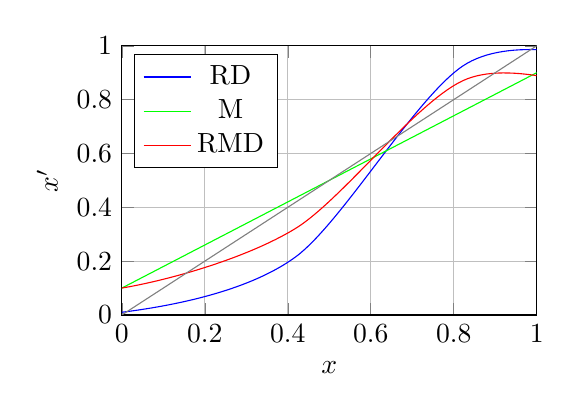
\begin{tikzpicture}
      \begin{axis}[xlabel=$x$, ylabel = $x'$,
                   grid=major, width=6.85cm, height = 5cm,
                   legend style = {legend pos = north west},
                   ymin=0,ymax=1, xmin=0,xmax=1]

      \addplot[smooth, color=blue] {x^2 / (3*x^2 - 4*x + 2) + 0.01};
      \addplot[smooth, color=green] {.8*x + .1};

      \addplot[smooth, color=red] {(.9*x^2 - .2*x +.2)/(3*x^2 - 4*x + 2)};

      \addplot[smooth, color=gray] {x};

      \legend{RD, M, RMD}

      \end{axis}
    \end{tikzpicture}


        \caption{Update functions: the population state $x$ is mapped onto $x'$ in one update step}
        \label{fig:Updates_RMS}
    \end{subfigure}
    \hfill
    \begin{subfigure}[b]{0.5\textwidth}    
      \centering
    \begin{tikzpicture}[x=120]
      \node[draw=black, circle, fill = black, minimum size = 0.25cm]
      (0) at (0,0) {};

      \node[draw=black, circle, fill = black, minimum size = 0.25cm]
      (1) at (1,0) {};

      \draw[-, thick] (0) -- (1);

      \node[draw=black, circle, fill = white, minimum size = 0.25cm, thick]
      (mid) at (2/3,0) {};

      \node[]  (0.label) at (0,-0.5) {0};

      \node[]  (1.label) at (1,-0.5) {1};

      \node[]  (label) at (0.5,-0.5) {$x$};

      \node[]  (label) at (0.5,0.55) {RD};

      \draw[->-=0.8,very thick] (mid) -- (0);

      \draw[->-=0.8,very thick] (mid) -- (1);

    \end{tikzpicture}
    
    \vspace*{1cm}

    \begin{tikzpicture}[x=120]

      \node (0) at (-0.05,0) {};

      \node (1) at (1.05,0) {};

      \node[draw=black, circle, fill = black, minimum size = 0.25cm]
      (S0) at (0.121,0) {};

      \node[draw=black, circle, fill = black, minimum size = 0.25cm]
      (S1) at (0.903,0) {};

      \draw[-, thick] (0) -- (1);

      \node[draw=black, circle, fill = white, minimum size = 0.25cm, thick]
      (mid) at (0.609,0) {};

      \node[]  (0.label) at (0,-0.3) {0};

      \node[]  (1.label) at (1,-0.3) {1};

      \node[]  (label) at (0.5,-0.5) {$x$};

      \node[]  (label) at (0.5,0.55) {RMD};

      \draw[->-=0.5,very thick] (mid) -- (S0);

      \draw[->-=0.5,very thick] (mid) -- (S1);

      \draw[->-=0.5,very thick] (0) -- (S0);

      \draw[->-=0.5,very thick] (1) -- (S1);

    \end{tikzpicture}
        


    \caption{Phase portraits for RD and RMD: unstable rest points are hollow, attractors are
      solid.}
        \label{fig:Phase_RD}
    \end{subfigure}

  \caption{Example}
  \label{fig:Example_RMD}
\end{figure}

While this was only an abstract and simple example, our goal is to apply the RMD to a more
complex case of co-evolving of lexical concepts and pragmatic behavior. To do so, we need to
fix three things: (i) what the relevant types are, (ii) how fitness derives from communicative
success and (iii) how the mutation matrix is computed. These issues are addressed, one by one,
in the following.

\subsection{Types: Lexica and linguistic behavior}
\label{sec:languages+use}

Types are what cultural evolution operates on. In standard applications of evolutionary game
theory, types correspond to ways of acting in a game, e.g., either cooperating or defecting in
a prisoner's dilemma. \mf{maybe good to refer back to the example from before if there was
  one?} \tb{Yes!} For our present purpose types are identified by their cognitive make-up. Since we are
interested in the question under which conditions processes of cultural evolution will favor
specific divisions of labor between lexical meaning and pragmatic use, a type is a pair
consisting of a lexicon and a pragmatic strategy.

Lexica codify the truth-conditions of expressions. A convenient way to represent lexica is by
$(\card{\States}, \card{\Messgs})$-Boolean matrices, where $\States$ is a set of states
(meanings) and $M$ a set of messages (forms available in the language). For example, suppose
that there are two relevant world states $\States = \set{\ssome, \sall}$. In state $\ssome$
Chris owns some but not all of Johnny Cash's albums while in $\sall$ Chris owns them
all. Suppose that there are two messages $\Messgs = \set{\msome, \mall}$ where $\msome$ is
short for a sentence like \emph{Chris owns some of Johnny Cash's albums} and $\mall$ for the
same sentence with \emph{some} replaced by \emph{all}.  
Lexica for this case would assign a Boolean truth value, either $0$ for false or $1$ for true, to each state-message pair. The following two lexica exemplify the distinction
between a lexicalized upper-bound for \emph{some} in $\Lbound$ and the widely assumed logical
semantics with only a lower-bound in $\Llack$.

\begin{align*}
  \Lbound & = \begin{blockarray}{lcc}
    & \mygray{\msome} & \mygray{\mall} \\
    \begin{block}{l[cc]}
      \mygray{\ssome} & 1 & 0 \\
      \mygray{\sall}  & 0 & 1 \\
    \end{block}
  \end{blockarray} &
  \Llack & = \begin{blockarray}{lcc}
    & \mygray{\msome} & \mygray{\mall} \\
    \begin{block}{l[cc]}
      \mygray{\ssome} & 1 & 0 \\
      \mygray{\sall}  & 1 & 1 \\
    \end{block}
  \end{blockarray}
\end{align*}

We distinguish between two kinds of linguistic behavior. {\em Literal interlocutors} produce and
interpret messages literally, being guided only by their lexica. {\em Pragmatic interlocutors}
instead engage in mutual reasoning to inform their choices. Recent probabilistic models of
rational language use
\citep{franke:2009,frank+goodman:2012,FrankeJager2015:Probabilistic-p,GoodmanFrank2016:Pragmatic-Langu}
capture different types of pragmatic behavior in a reasoning hierarchy. The hierarchy's bottom,
level $0$, corresponds to literal language use. Pragmatic language users of level $n + 1$
act (approximately) rational with respect to level-$n$ behavior of their
interlocutors. (\ref{h:level0}) and (\ref{s:level0}) define probabilistic behavior of literal
hearers and speakers respectively: \mf{is it a problem that $S$ denotes speakers and the set of
states?} \tb{I think that's fine. $S_n(\cdot \mid \cdot)$ is not used beyond this section. Otherwise we can, e.g., relabel $M$ as $F$(orms) and use $M$(eanings) instead of $S$(tates). I'm fine with either option.}
\begin{flalign}
&H_{0}(s \mid m;L) \propto pr(s) L_{sm} \label{h:level0}\\
&S_{0}(m \mid s;L) \propto \exp(\lambda \; L_{sm}) \label{s:level0}
\end{flalign}

According to (\ref{h:level0}), a literal hearer's interpretation of a message $m$ as a state
$s$ depends on her lexicon and her prior over states, $pr \in \Delta(S)$. For simplicity, in
the following this prior is assumed to be uniform. A literal interpreter with lexicon $\Lbound$
from above would assign $\ssome$ a probability of $H_0(\ssome \mid \msome; \Lbound) = 1$ after
hearing $\msome$, while a literal interpreter with lexicon $\Llack$ would assign $\ssome$
probability $H_0(\ssome \mid \msome; \Llack) = 0.5$. As usual in probabilistic pragmatics models, speaker behavior is regulated by a soft-max
parameter $\lambda$, $\lambda \geq 1$ \citep{luce:1959,sutton+barto:1998}. As $\lambda$
increases, choices made in production are more rational in that they are increasingly in line with expected utility maximization. Expected utility of a message
$\messg$ in state $\state$ for a level $n+1$ speaker is here defined as $H_{n}(s|m;L)$, the probability that the hearer will assign to or choose the correct meaning. Put differently, expected utility indicates how likely the hearer is thought to infer $\state$ when sent $\messg$. The formulation
in (\ref{s:level0}) also allows false messages to be sent with a small positive probability in
analogy to the definition of pragmatic speakers in probabilistic pragmatic models. This is also necessary to guarantee a mutation matrix with only positive entries (see below). If $\lambda = 1$ a literal
speaker with either lexicon $\Lbound$ or $\Llack$ produces $\msome$ in $\ssome$ with probability $S_{0}(\msome \mid
\ssome;L_{\text{bound},\text{lack}}) \approx .73$. The probability of producing $\msome$ in $\sall$ is $S_{0}(\msome \mid
\sall;\Lbound) \approx .27$ for $\Lbound$ and $S_{0}(\msome \mid
\sall;\Llack) = .5$ for $\Llack$. By contrast, if $\lambda = 20$, a literal speaker with either lexicon produces $\msome$ in $\ssome$ with probability $S_{0}(\msome \mid
\ssome;L_{\text{bound},\text{lack}}) \approx 1$. But the probability of producing $\msome$ in $\sall$ is $S_{0}(\msome \mid
\sall;\Lbound) \approx 1$ for $\Lbound$ whereas it is still $S_{0}(\msome \mid \sall;\Llack) = .5$ for $\Llack$ because it semantically associates $\msome$ with both states.

Pragmatic behavior of level $n+1$ is similar to its literal counterparts but bases linguistic choice in 
interpretation or production on the expected behavior of a level-$n$ interlocutor instead of on lexical meaning:
\begin{flalign}
&H_{n+1}(s|m;L) \propto pr(s) S_{n}(m|s;L) \label{h:leveln}\\
&S_{n+1}(m|s;L) \propto  \exp(\lambda \; H_{n}(s|m;L)) \label{s:leveln}
\end{flalign}

Particularly important to our purpose is the fact non-literal interlocutors using $\Llack$ can {\em pragmatically} associate $\msome$ with $\ssome$ over $\sall$,  in contrast to their literal counterparts. Intuitively, this is so because hearers reason a speaker to convey $\sall$ with $\mall$, as this message has a higher chance of leading to mutual understanding than using underspecified $\msome$. Therefore they will expect $\msome$ to be more strongly associated with $\ssome$ than with $\sall$ as it is already possible to clearly convey the latter state $\mall$. The converse reasoning pattern holds for the speaker. In this way, two distinct lexical conventions such as $\Lbound$ and $\Llack$ can give rise to similar observable linguistic behavior. In this case, associating $\msome$ with $\ssome$ and $\mall$ with $\sall$.

\subsection{Fitness \& fitness-based selection based on expressivity}\label{sec:expressivity}

Most evolutionary dynamics assume that the proportion of type $i$ in a population will increase
or decrease as a function of its relative fitness $f_i$. In the context of language evolution,
fitness is frequently associated with expressivity, i.e., the ability to successfully
communicate with other language users from the same population
\citep[e.g.,][]{nowak+krakauer:1999,nowak+etal:2000, nowak+etal:2002}. Under a biological
interpretation the assumption is that organisms have a higher chance of survival and
reproduction if they are able to share and receive useful information via communication with
peers. Under a cultural interpretation the picture is that agents themselves strive towards
communicative success and therefore occasionally adapt or revise their behavior to achieve a
higher communicative success (see \citealt[\S3.3]{benz+etal:2005b} for discussion).

The replicator equation gives us the means to make the ensuing dynamics precise, without
necessarily committing to a biological or cultural interpretation. As above, the proportion of types in a
given population is codified in a vector $\vec{x}$, where $x_i$ is type $i$'s proportion. The
fitness of type $i$ is its average expected communicative success, or \emph{expected
  utility} (EU), given the frequencies of types in the current population:
\begin{align*}
  f_i = \sum_j x_j \text{EU}(t_i,t_j)\,.
\end{align*}
The expected utility $\text{EU}(t_i,t_j)$ for type $i$ when communicating with type $j$ is the
average success of $i$ when talking or listening to $j$. Assuming that agents are speakers half
of the time, this yields:
\begin{align*}
  \text{EU}(t_i,t_j) = \nicefrac{1}{2} \, \text{EU}_S(t_i,t_j) + \nicefrac{1}{2} \, \text{EU}_H(t_i,t_j)\,,
\end{align*}
where $\text{EU}_S(t_i,t_j)$ and $\text{EU}_H(t_i,t_j)$ are the expected utilities for $i$ as a
speaker and as a hearer when communicating with $j$, defined as follows, where $n_i$ and $n_j$
are type $i$'s and type $j$'s pragmatic reasoning types and $L_i$ and $L_j$ are their lexica:
\begin{flalign*}
  & \text{EU}_S(t_i,t_j)  = \sum_s P(s)\sum_m S_{n_i}(m \mid s;L_i) \sum_{s'} R_{n_j}(s' \mid m;L_j)
  \delta(s,s') \\
 & \text{EU}_H(t_i,t_j)  = \text{EU}_S(t_j,t_i)
\end{flalign*}
As usual for cooperative communication, $\delta(s,s') = 1$ iff $s = s'$ and $0$ otherwise.

\subsection{Learnability}
\label{sec:learnability}

Languages are shaped not only by functionalist forces towards greater expressivity. Another
important factor is the fidelity by which language is transmitted. Among others, linguistic
production can be prone to errors, states or messages may be perceived incorrectly, and
multiple languages may be compatible with the data learners are exposed to. These sources of
uncertainty introduce variation in the transmission of linguistic knowledge from one generation to the next. In particular, learning biases in the iterated transmission process can influence language evolution
substantially.

In biological evolution, where types are expressed genetically, transmission infidelity comes
into the picture through infrequent and mostly random genetic mutations. However, an agent's lexicon
and pragmatic reasoning behavior is not inherited genetically. They need to be learned from
observation. Concretely, when agents of type $j$ want to adopt or imitate the linguistic
behavior of type $i$, they observe the overt linguistic behavior of type $i$ and need to infer what
their type is from that. Iterated learning is a process in which languages are learned repeatedly from the observation
of linguistic behavior of agents who have acquired the language from observation and inference
before as well. In the simplest case there is a single teacher and a single
learner. After sufficient training the learner becomes a teacher and produces behavior that
serves as input for a new learner. Due to the pressure towards learnability it exerts, iterated
learning alone generally leads to simpler and more regular languages (see \citealt{kirby+etal:2014}
and \citealt{tamariz+kirby:2016} for recent surveys). 

Following \citet{griffiths+kalish:2007} we model language acquisition as a process of Bayesian
inference in which learners combine the likelihood of a type producing the witnessed learning
input with prior inductive biases. Experimental and mathematical results on iterated learning
suggest that the outcome of this process reflects learners' inductive biases
\citep[e.g.,][]{kirby+etal:2014}. In a Bayesian setting these biases can be codified in a prior
$P \in \Delta(T)$, which reflects the amount of data a learner requires to faithfully acquire
the language of the teacher \citep[cf.][450]{griffiths+kalish:2007}. The extent of the prior's
influence has been shown to heavily depend on the learning strategy assumed to underlie the
inference process. On the one hand, early simulation results suggested that weak biases could
be magnified by exposing learners to only small data samples \citep[e.g. in][]{brighton:2002}. On the other, \citeposs{griffiths+kalish:2007} mathematical
characterization showed that iterated learning converged to the prior, i.e., that the resulting
distribution over languages corresponds to the learners' prior distribution and is not
influenced by the amount of input given to them. This difference in predictions can be traced
back to differences in the selection of hypotheses from the posterior. Griffith \& Kalish's
convergence to the prior holds for learners that sample from the posterior. More deterministic
strategies such as the adoption of the type with the highest posterior probability, so-called
{\it maximum a posterior estimation} (MAP), increase the influence of both the prior and the
data \citep{griffiths+kalish:2007,kirby+etal:2007}. In the following, we use a parameter
$l\ge1$ to modulate between posterior sampling and the MAP strategy. When $l = 1$ learners
sample from the posterior. The learners' propensity to maximize the posterior grows as $l$
increases.

Let $D$ be the set of possible data that learners may be exposed to. This set $D$ contains all
sequences of state-message pairs of length $k$, e.g.,
$\tuple{\tuple{s_1,m_1},\dots , \tuple{s_k,m_k}}$. As $k$ increases, learners have more data to base their inference on and so tend to
recover the true types that generated a given sequence with higher probability. The mutation
matrix $Q$ of the replicator mutator dynamics in (\ref{eq:RMD_discrete}) can then be defined as
follows: $Q_{ji}$ is the probability that a learner acquires type $i$ when learning from an
agent of type $j$. The learner observes a length-$k$ sequence $d$ of state-message pairs, but
the probability $P(d \mid t_j)$ with which sequence $d = \tuple{\tuple{s_1,m_1},\dots , \tuple{s_k,m_k}}$ is observed depends on type $j$'s
behavior:
\begin{align*}
  P(d = \tuple{\tuple{s_1,m_1},\dots , \tuple{s_k,m_k}} \mid t_j) = \prod_{i = 1}^k S_{n_j}(m_i
  \mid s_i; L_{j})\,,
\end{align*}
where, as before, $n_j$ is $j$'s pragmatic reasoning type and $L_j$ is $j$'s lexicon. For a
given observation $d$, the probability of acquiring type $i$ is $F(t_i \mid d)$, so that:
\begin{flalign*}
  Q_{ji} \propto \sum_{d \in D} P(d \mid t_j) F(t_i \mid d)\,.
\end{flalign*}
The acquisition probability $F(t_i \mid
d)$ given datum $d$ is obtained by probability matching $l = 1$ or a tendency towards choosing
the most likely type $l > 1$ from the posterior distribution $P(\cdot \mid d)$ over types given
the data, which is calculated by Bayes' rule:
\begin{flalign*}
  & F(t_i \mid d) \propto P(t_i \mid d)^l \; \text{ and }\\
  & P(t_i \mid d) \propto P(t_i) P(d \mid t_i)\,.
\end{flalign*}


\subsection{Model summary}

Expressivity and learnability are central to the cultural evolution of language. These
components can be modelled, respectively, as replication based on a measure of fitness in terms
of communicative efficiency and iterated Bayesian learning. Their interaction is described by
the discrete time replicator mutator dynamics in (\ref{eq:RMD_discrete}), repeated here:
\begin{align*}
  x'_i = \sum_j Q_{ji} \frac{x_jf_j}{\sum_k x_k f_k}\,.
\end{align*}
This equation defines the frequency $x'_i$ of type $i$ at the next time step, based on its
frequency $x_i$ before the step, its fitness $f_i$, and the probability that a learner infers
$i$ when observing the behavior of a type-$j$ agent. Fitness-based selection can be thought of
as biological (fitness as expected relative number of offspring) or cultural (fitness as 
likelihood of being imitated or repeated). The types that the dynamic operates on are pairs
consisting of a lexicon and a pragmatic use pattern. A type's expressivity depends on its
communicative efficiency within a population while its learnability depends on the fidelity by
which it is inferred by new generations of learners. The learners' task is consequently to
perform a joint inference over types of linguistic behavior and lexical meaning.


\section{Scalar implicatures}\label{sec:si-case-study}
%
Scalar implicatures are a particularly well-studied type of conventional pragmatic inferences. They are licensed for groups of expressions ordered in terms of informativity, here understood as an entailment induced order. For instance, {\em some} is entailed by {\em all}. If it were true that ``Chris owns all of Johnny Cash's albums'', it would also be true that ``Chris owns some of Johnny Cash's albums''. However, while weaker expressions such as {\em some} are truth-conditionally compatible with stronger alternatives such as {\em all}, this is not what their use is normally taken to convey. Instead, the use of a less informative expression when a more informative one could have been used can license a defeasible inference that stronger alternatives do not hold (cf. \citealt{horn:1972,gazdar:1979}). That is, a hearer who assumes the speaker to be able and willing to provide all relevant information can infer that stronger alternatives do not hold because the speaker used a weaker alternative instead. In this way, ``Chris owns some of Johnny Cash's albums'' is strengthened to convey that he owns {\em some but not all} albums. A bound that rules out stronger alternatives is thusly not codified in the lexical meaning of weak alternatives but instead pragmatically supplied.

As noted earlier, this kind of strengthening is captured by the linguistic behavior of pragmatic types introduced in \S\ref{sec:languages+use}: A pragmatic hearer who reasons about the use of a message involving a weak scalar alternative will associate it more with a state in which stronger alternatives do not hold. This is so because a rational speaker would use a more informative message when in such a state. Conversely, a pragmatic speaker will reason about her interlocutor's expected interpretation and use the messages at her disposition accordingly as to maximize communicative success.

Our initial question about the division of labor between semantics and pragmatics can be narrowed to the case of scalar implicatures by asking for a justification for the lack of lexical upper-bounds in weak scalar alternatives. That is, we ask why lexical meanings that lack upper-bounds and convey it pragmatically are regularly selected for over alternatives such as that of codifying the bound semantically. More poignantly, would it not serve language users better if weak(er) expressions such as {\em warm}, {\em or}, {\em some} and {\em big} were truth-conditionally incompatible with stronger alternatives such as {\em hot}, {\em and}, {\em all} and {\em huge} to avoid misunderstanding?  This question is particularly striking considering the number of expressions that license such inferences across natural languages. 

We see two main explanations for the lack of upper-bounds in the lexical meaning of weak scalar expressions. The first is that their truth-conditional compatibility with stronger expressions endows them with a broader range of applicability by allowing them to occur in contexts in which their upper-bounded reading is absent. This can happen when embedded in downward-entailing contexts, when the speaker is likely uncertain about whether the upper bounded reading is true, or when the distinction between an upper-bounded reading and the simple, only lower-bounded reading, is not relevant. For instance, if for all the speaker knows Chris owns some of Johnny Cash's albums but she does not know whether he owns all, then the use of {\em some} lacking an upper-bound succinctly conveys her uncertainty. This may suggest a functionalist argument for why upper-bounded meanings do not conventionalize: Should contextual cues provide enough information to the hearer to identify whether a bound is intended to be conveyed pragmatically, then this is preferred over expressing it overtly through longer expressions, e.g., by saying {\em some but not all} explicitly. Importantly, although morphosyntactic disambiguation may be dispreferred due to its relative length and complexity \citep{piantadosi+etal:2012b}, it allows speakers to enforce an upper-bound and override contextual cues that might otherwise mislead the hearer. In a nutshell, this explanation posits that scalar implicatures fail to lexicalize because, all else being equal, speakers prefer to communicate as economically as possible and pragmatic reasoning enables them to do so. Compare this with a hypothetical language that lexicalizes two expressions for each weak scalar expression -- one with and one lacking an upper-bound. We see four conditions along this functionalist explanation that may pressure languages for English-like semantics over this alternative. First, contextual cues are very reliable. Second, morphosyntactic disambiguation is seldom necessary. Third, morphosyntactic disambiguation is only marginally dispreferred. Fourth, larger lexica are costly. Overall, neither condition seems convincing as a central explanatory device for such a widespread phenomenon. The first two conditions put a heavy burden on the ability to retrieve contextual cues to a degree that seems unlikely to undercut the benefit of unambiguous communication. It is likely that human language users are very good at retrieving cues from context, but to stipulate that they are so good as to undercut the benefit of safe communication provided by this hypothetical alternative strikes us as too strong of an assumption.  As for the third and fourth condition, these seem mostly like technical solutions without a proper empirical basis. 

Instead, the systematicity and typological spread of scalar implicatures together with the observation that monomorphemic expressions that lexically rule out stronger alternatives are unattested across languages (\citealt[252-267]{horn:1984}, \citealt{horn:1972,traugott:2004,vdAuwera:2010}) suggests that other forces may be at play. In what follows we investigate the predictions of our model under the assumption that the lack of lexicalization of scalar inferences may be accounted for by the relative representational simplicity of lexical meanings lacking an upper-bound over those that explicitly codify it. This difference is reflected in a learning bias towards more compressed lexical representations. That is, in a preference of learners for simpler over more complex explanations of the data they witness \citep{feldman:2000, chater+vitanyi:2003, piantadosi+etal:2012a, kirby+etal:2015,piantadosi+etal:underreview}. While we do not want to argue that functional aspects as the ones discussed above do not play a role, we do see a clear benefit in exploring whether matters of transmission biases would not give us additional explanatory leverage.


\subsection{Analysis}
The dynamics are initialized with an arbitrary distribution over types, constituting a population's first generation. In the following we report the outcome of their development under different parameters and pressures after $50$ generations. This ensures that these outcomes correspond to developmental plateaus after which no noteworthy change is registered. As specified in \S\ref{sec:learnability}, the mutation matrix $Q$ can be obtained by considering all possible state-message sequences of length $k$. Given that this is intractable for large $k$, the sets of data learners are exposed to are approximated by sampling $250$ $k$-length sequences from each type's production probabilities. 

We begin setting the stage by defining the learning prior and the set of types under consideration. Drawing from our preceding discussion, functional pressure on successful communication combined with learning pressures in the form of a bias that favors simpler semantics may lead to the selection of $\Llack$-like semantics and to a division of labor between semantics and pragmatics. We first showcase the effects that expressivity and learnability have in isolation before turning to those resulting from their combination. 


\subsubsection{An inductive learning bias for semantic simplicity}
There is a growing effort to develop empirically  testable representational  languages that allow for the measure of semantic complexity. For instance, so-called {\em languages of thought} (LOT) have been put to test in various rational probabilistic models that show encouraging results (see, e.g., \citealt{katz+etal:2008, piantadosi+etal:underreview, piantadosi+etal:2012a} and \citealt{piantadosi+jacobs:2016} for recent discussion). At its core, a LOT defines a set of operations and composition rules from which lexical meaning can be derived. As a first approximation and for the sake of concreteness, we follow this approach to make the preference of learners for simpler semantic representations precise and define the complexity of a representation as a function of its derivation cost in a weighed generative LOT.

Our toy grammar of concepts is given in Table~\ref{tab:grammar}. This grammar uses basic set-theoretic operations to form expressions which can be evaluated as true or false in different world states such as $\ssome$ or $\sall$. Applications of generative  rules have a cost attached to them. Here we simply assume that Boolean combinations of concepts are more complex than atomic concepts and that otherwise each rule application adds the same cost unit.
\begin{table}
  \centering
  \begin{align*}
    C & \rightarrow_2 C \wedge C 
    & 
    X & \rightarrow_1 \set{A,B} \\
    C & \rightarrow_2 \neg C 
    & 
    X & \rightarrow_1 X \cap X \\
    C & \rightarrow_1 X \subseteq X
    & 
    X & \rightarrow_1 X \cup X \\
    C & \rightarrow_1 X \neq \emptyset \\
    C & \rightarrow_1 X = \emptyset     
  \end{align*}
  \caption{Toy grammar in a set-theoretic LOT with weighted rules.}
  \label{tab:grammar}
\end{table}


The prior probability of a type is just the prior probability of its lexicon. The prior of a lexicon is a function of the complexity of the lexical representations in its image set. As motivated above, lexica that use simpler concepts are \emph{a priori} more likely. A simple way of defining such priors over lexica is:
\begin{align*}
  P(L)  & \propto \prod_{c \in Im(L)} P(c)   \ \text{, with} & 
  P(c) & \propto \max_{c'}Compl(c') - Compl(c) + 1\,,
\end{align*}

where $Compl(c)$ is the complexity of the minimal derivation length of $c$ according to the LOT-grammar. There are many ways to define priors over lexica (see, e.g., \citealt{goodman+etal:2008, piantadosi+etal:2012a}) but the key assumption here, common to all of them, is that simple representational expressions should be favored over more complex ones. We should stress that these details -- from the generative grammar to its complexity measure -- are to be regarded as an instantiation of our general assumptions instead of as empirical claims in their own right. 




\subsubsection{Lexica, signaling behavior \& types}
We consider a state space with three states $\States = \set{\snone, \ssome, \sall}$. \tb{Should we say something about the inclusion of $\snone$? It may be more natural to introduce this state earlier but may unnecessarily complicate the exposition of signaling behavior in the previous section.} This space can be
thought of as a partition of possible worlds into cells where none, some or all of the $A$s are
$B$s, for some arbitrary fixed predicates $A$ and $B$. Eight concepts can be distinguished
based on their truth or falsity in three world states, six of which are not contradictory
 or tautological. These are listed with mnemonic names in
Table~\ref{tab:concepts} together with their complexity according to the grammar in Table \ref{tab:grammar}.

\begin{table}
  \centering
\begin{center}
  \begin{tabular}{lccclc}
    \toprule
    intuitive name
    & \snone
    & \ssome
    & \sall
    & least complex formula
    & complexity
    \\ \midrule
    ``all''
    & 0
    & 0
    & 1
    & $A \subseteq B$
    & $3$
    \\
    ``some but not all''
    & 0
    & 1
    & 0
    & $A \cap B \neq \emptyset \wedge A \neq \emptyset$
    & $8$
    \\    
    ``some''
    & 0
    & 1
    & 1
    & $A \cap B \neq \emptyset$
    & $4$
    \\
    ``none''
    & 1
    & 0
    & 0
    & $A \cap B = \emptyset$
    & $4$
    \\
    ``none or all''
    & 1
    & 0
    & 1
    & $\neg(A \cap B \neq \emptyset \wedge A \neq \emptyset)$
    & $10$
    \\
    ``not all''
    & 1
    & 1
    & 0
    & $\neg (A \subseteq B)$
    & $5$
    \\
    \bottomrule
  \end{tabular}
\end{center}
\caption{Available concepts and their minimal derivation length}
\label{tab:concepts}
\end{table}

A lexicon $L$ is a mapping $\Messgs \rightarrow C$ from messages to concepts. With three
messages there are $6^3 = 216$ possible lexica. Some assign the same concept to more than one message and others lexicalize the same concepts but associate them with different messages. The main results reported in the following do not hinge on the inclusion of these lexica but this unaltered space does better illustrate the influence and differences of the linguistic pressures we consider. Additionally, the competition of different languages that lexicalize the same concepts through different forms allows us to take serious the problem of only one being selected for even though multiple alternatives of equal expressivity {\em and} learnability exist.

Out of these possible lexica, three kinds are of particular relevance. First, lexica that assign the same concept to more than one message. Such lexica lack in expressivity but may be favored by the learning prior should they lexicalize simple concepts. Second, lexica that conventionalize upper-bounds to realize a (quasi-)partition of the state space. As discussed before in relation to $\Lbound$, users of these lexica need not resort to pragmatic reasoning to convey an upper-bound with weak scalar expressions. Instead, this information is already provided by the semantics of their lexicon, giving them an advantage in terms of expressivity. Types with such lexica are expected to be the main contenders of the natural language like semantics that do not lexicalize an upper-bound for weak scalar expressions. Third and lastly, $\Llack$-style lexica that, paired with mutual reasoning, can convey an upper-bound pragmatically. There are six lexica of the second kind and six of the third. The following three lexica exemplify each kind, with $\Lall$ being a lexicon of the first kind. This lexicon is not optimal for communication as it assigns all its messages to the same state, $\sall$. This inevitably leads to a communicative disadvantage in its use. However, it may have a learnability advantage over our target $\Llack$ and its competitor $\Lbound$ in virtue of being the simplest lexicon, making it a priori favored by learners.

\begin{align*}
  \begin{blockarray}{lccc}
    & & \underline{\Lall} & \\
    & \mygray{\mnone} & \mygray{\msome} & \mygray{\mall} \\
    \begin{block}{l[ccc]}
     \mygray{\snone}  & 0 & 0 & 0\\
     \mygray{\ssome}  & 0 & 0 & 0\\
    \mygray{\sall}   & 1 & 1 & 1\\
    \end{block}
% \\ & & P(\Lall)\rlap{ $\propto 9$} & \\
  \end{blockarray} & &
 \begin{blockarray}{lccc}
    & & \underline{\Lbound} & \\
    & \mygray{\mnone} & \mygray{\msome} & \mygray{\mall} \\
    \begin{block}{l[ccc]}
       & 1 & 0 & 0\\
       & 0 & 1 & 0\\
       & 0 & 0 & 1\\
    \end{block}
%  \\& & P(\Lbound)\rlap{ $\propto 96$} & \\
  \end{blockarray} & &
  \begin{blockarray}{lccc}
    & & \underline{\Llack} & \\
    & \mygray{\mnone} & \mygray{\msome} & \mygray{\mall} \\
    \begin{block}{l[ccc]}
       & 1 & 0 & 0\\
       & 0 & 1 & 0\\
       & 0 & 1 & 1\\
    \end{block}
%   \\& & P(\Llack)\rlap{ $\propto 48$} & \\
  \end{blockarray}
\end{align*}



Recall that types are a combination of a lexicon and a manner of language use. We analyze the model's predictions in populations of types with one of the two behaviors introduced earlier; literal or pragmatic. The former correspond to level $0$ reasoners and the latter to ones of level $1$. Higher level reasoning is not required to derive scalar implicatures from these lexica, nor do they leave room for substantial pragmatic refinement. Accordingly, we consider a total of $432$ types. Six are variants of our pragmatic $\Llack$ target and twelve are either literal or pragmatic speakers of variants of its main contender, $\Lbound$.

%Combining a linguistic behavior with each of these $6$ lexica yields a total of $12$ distinct types. , such as $L_4$, will produce speaker behavior that is {\em almost} indistinguishable from that of a language that lacks upper-bounds, but with pragmatic users, such as $L_5$. Almost, because there may be slight differences between the probability with which speakers would (erroneously) use a semantically false description and the probability with which speakers would (erroneously) use a pragmatically suboptimal description. Due to this possibly marginal difference between pragmatic $L_4$ and $L_5$, the selection of one type over the other is expected to mainly depend on how well each can be transmitted to new learners. Things are less clear for literal $L_5$ contrasted with literal/pragmatic $L_4$. The former has a learning advantage when learners are biased against upper-bounds but is expected to fare worse in communicative terms.

\subsubsection{Expressivity only} 
\begin{figure}
\centering
\includegraphics[width=\textwidth,height=8cm, keepaspectratio]{./plots/fig1-onlyr}
\caption{Stacked proportion of pragmatic $\Llack$-style types and incumbent types, when other than pragmatic $\Llack$, in $5$ independent populations after $50$ generations under only a pressure for expressivity. The right-most plots zoom in on only the proportion of pragmatic $\Llack$ types.}
\label{fig:only-R}
\end{figure}

Expressivity is sensitive to $\lambda$ as it influences signaling behavior. This is showcased in Figure \ref{fig:only-R}, which depicts the proportion of pragmatic $\Llack$-style speakers in $5$ independent populations after $50$ generations, as well as that of the type with the highest proportion in a given population, the incumbent. Low $\lambda$ levels communicative differences between types, as even those that can differentiate between all states semantically or pragmatically do not always maximize expected communicative success. The outcome is that of a mixed population that allows for the survival of competing types. Conversely, higher $\lambda$ promotes more rational linguistic behavior, widening the gap in expressivity between types and promoting more homogeneous populations. As suggested by Figure \ref{fig:only-R}, the incumbent in most populations is not one of the six pragmatic $\Llack$-style types. That is, a pressure only for expressivity does not lend a justification to the systematic prevalence of a lack of upper-bounds under any $\lambda$-value. For instance, in $1000$ independent populations with $\lambda = 20$ pragmatic $\Llack$ types only made up $11$ cases of incumbency, corresponding to a mean proportion of $0.003$ across populations. By contrast, $913$ incumbents were $\Lbound$-style users with close to an even share between literal ($454$) and pragmatic types ($459$), corresponding to a mean proportion of about $.48$ taken together. %Across types and populations incumbents make up $.50$ of the mean outcome. 


\subsubsection{Learnability only}

\begin{figure}
\centering
\includegraphics[width=1\textwidth,height=8cm,keepaspectratio]{./plots/fig2-onlym-pr}
\caption{Stacked proportion of pragmatic $\Llack$-style types and incumbent types, when other than pragmatic $\Llack$, in $5$ independent populations after $50$ generations under only a pressure for learnability ($\lambda = 20, k = 5$). The types' prior probability is shown in the right-most plot.}
\label{fig:only-M}
\end{figure}

The effect of iterated learning without a pressure for expressivity using either posterior sampling ($l = 1$) or a stronger tendency towards posterior maximization ($l = 15$) is shown in Figure \ref{fig:only-M} together with the prior over types. The prior shows that while users of $\Llack$ are not the most favored by the inductive bias (compared, e.g., to $\Lall$) they are nevertheless more advantaged than others, such as $\Lbound$, in virtue of the relatively simple semantics they conventionalize. Crucially, $\Llack$ enables its users to convey each state with a single message when combined with pragmatic reasoning provided sufficiently high $\lambda$. This makes it less likely to be confused with other types if the learning data is not too sparse ($k \geq 5$). Put differently, learners have a higher propensity to infer pragmatic $\Llack$ over types that might be hard or impossible to distinguish it from based on overt linguistic behavior, such as $\Lbound$, and $\Llack$ is also less likely to be mistaken with types with different observable behavior because its pragmatic use approximates a one-to-one form-meaning mapping. As a consequence, a stronger propensity to maximize the posterior increases their proportion in the population. 

However, in contrast to a pressure only for expressivity with high $\lambda$, learnability alone does not succeed in selecting for a single type of a kind. For instance, for only one of the six pragmatic $\Llack$ types. Instead, it leads to their coexistence. Each is passed on to next generation with the same faithfulness and, differently from a pressure for communicative success, they do not stand in competition with each other. As implicit in Figure \ref{fig:only-M}, in $1000$ independent populations all incumbents were pragmatic $\Llack$ users provided sufficiently high $\lambda$, with each reaching approximately the same proportion of users in the population. As with expressivity only, low values of $\lambda$ make the differences in observable behavior across types less pronounced and therefore reflect the learners' inductive bias more faithfully, favoring functionally deficient but a priori preferred types such as those that use $\Lall$. A pressure for learnability alone may consequently lead to a spread of communicatively suboptimal types that are easier to learn. In the extreme, when $l = 1$ and $\lambda = 1$ all of $1000$ independent populations had users of $\Lall$ as incumbents.

\subsubsection{Expressivity and learnability}
The separate inspection of each pressure not only showcases the contribution of the model's components but also highlights some of their broader implications for the emergence of a division of labor between semantics and pragmatics. Neither dynamic on its own comes close to converging to a monomorphic population of pragmatic $\Llack$ speakers. When pressured toward expressivity, the slight communicative advantage of $\Lbound$'s lexicalization of an upper-bound over pragmatic use of $\Llack$ leads to the former's selection. When pressured toward learnability, pragmatic $\Llack$ is promoted over functionally similar but semantically more complex alternatives such as $\Lbound$. However, on its own learnability does not foment the propagation of these types across the population. What is more, it leads to heterogeneous populations that foster an equal share of types of a kind, such as different pragmatic $\Llack$ types.

\begin{figure}
\centering
\includegraphics[width=1\textwidth,height=8cm,keepaspectratio]{./plots/fig3-r+m}
\caption{Stacked proportion of pragmatic $\Llack$-style types and incumbent types, when other than pragmatic $\Llack$, in $5$ independent populations after $50$ generations under both pressures ($k = 5$).}
\label{fig:rmd}
\end{figure}

Figure \ref{fig:rmd} illustrates the combined effects of both pressures for a sample of $\lambda$ and $l$ values. These results show that an inductive learning bias for simpler semantics in tandem with functional pressure can lead to the selection of $\Llack$-like semantics paired with pragmatic language use. The proportion of these types increases with $\lambda$ and $l$. Pressure towards expressivity magnifies the effects of iterated learning and dampens the proliferation of types of a kind that are equal in expressivity {\em and} learnability. A pressure towards learnability favors the transmission of simpler semantics and thereby makes types that exploit pragmatic reasoning to strengthen lexical meaning more likely to be adopted over alternatives that do not. %In short, neither learnability nor functional pressure alone but their combination may lead to the lack of upper-bounds in the lexical meaning of scalar expressions in predominantly monomorphic populations. 

As before, low $\lambda$ and $l$ lead to the incumbency of communicatively suboptimal types that are a priori favored, such as $\Lall$. An increase in $\lambda$ leads to the selection and incumbency of pragmatic $\Llack$ but does not lead to monomorphic populations if learners sample from the posterior. Finally, a combination of sufficiently rational signaling behavior with some tendency for posterior maximization leads to increasingly monomorphic populations of types that convey upper-bounds pragmatically. The difference between the mean of the highest pragmatic $\Llack$-like type in $1000$ independent populations and the highest proportion of other types across $\lambda$ and $l$ values is shown in Figure \ref{fig:diff}.

\begin{figure}
\centering
\includegraphics[width=1\textwidth,height=6cm,keepaspectratio]{./plots/fig4-incumbents-difference}
\caption{Difference between mean proportion of highest pragmatic $\Llack$ type and highest other type in $1000$ independent populations after $50$ generations under both pressures ($k = 5$). \tb{I will run more simulations with higher $\lambda$ and $l$. I'm pretty sure the difference still increases.}}
\label{fig:diff}
\end{figure}

As for the effect of the sequence length $k$ not mentioned so far, it influences populations in a predictable way: small values lead to more heterogeneous populations that reflect the learner's prior more faithfully. This is due to the fact that the likelihood that a small sequence was produced by any type is relatively uniform (modulo prior). By contrast, larger values increasingly allow learners to differentiate types with different signaling behaviors.

To recapitulate, other than the involvement of both pressures, the resulting proportion of pragmatic $\Llack$ speakers primarily hinges on three factors. First, the degree to which agents try to maximize communicative success. This plays a role both in expressivity as well as in producing data that allows learners to discriminate this type from others. Second, the inductive bias, which leads learners to prefer simpler over more complex semantic representations in acquisition. Lastly, the posterior parameter, as it magnifies the effects of the learning bias in tandem with replication. 




\subsection{Discussion}
Under the assumption of a learning bias for simpler lexical representations, our results suggest that a lack of semantic upper-bounds coupled with pragmatic reasoning can overcome communicative pressures and be majoritarily selected for in a population. This prediction hinges on three assumptions. First, that language is pressured toward both expressivity and learnability. Second, that language users favor expressions/interpretations expected to have a higher likelihood of being understood/meant over ones with a lower likelihood. Lastly, that learners prefer simpler over more complex lexical representations and exhibit a tendency towards the acquisition of the type that best explains the learning data. This outcome is particularly encouraging in light of other advantages a lack of semantic upper-bounds may confer, as discussed at the beginning of this section.

A lack of upper-bounds in the lexical meaning of weak scalar expressions constitutes the majority view in the literature. However, it not clear to what extent other types should be present in the final population. It seems reasonable to expect functionally suboptimal lexica such as $\Lall$ to be ruled out but matters are different for $\Lbound$. The prediction that natural language communities are homogeneous or that speakers may entertain $\Llack$-like semantics for one scalar expression and $\Lbound$-like semantics for another is not implausible (cf. \citealt{franke+degen:2016}). Alternatively, a stronger tendency for posterior maximization in learning has to be assumed. This empirical issue relates to other two aspects left undiscussed: disadvantages of pragmatic reasoning and the effect of state frequencies on the fossilization of pragmatic inferences. We tacitly assumed pragmatic reasoning to come at no cost. However, there is experimental evidence that suggests  that the pragmatic derivation of upper-bounds costs effort and takes additional processing time (cf. \citealt{deNeys+schaeken:2007, huang+snedeker:2009}). This raises the question at which point such usage-based cost undercuts the learnability advantage of simpler semantic representations. Should cost play a role, then its effect is bound to depend on the frequency with which a given scalar expression is used. It may be that frequently drawn scalar implicatures fossilize to avoid cost whereas infrequent ones are derived on-line to avoid complexity in acquisition. This also opens a possible venue to address the preceding question about the expected presence of $\Lbound$-like semantics in a population, but further empirical evidence is needed to assess these matters.


\section{General discussion}\label{sec:discussion}
We laid out a model that combines game theoretical models of functional pressure towards efficient communication \citep{nowak+krakauer:1999}, effects of transmission perturbations on (iterated) language learning \citep{griffiths+kalish:2007}, probabilistic speaker and listener types of varied degrees of pragmatic sophistication \citep{frank+goodman:2012, franke+jaeger:2014} as well as different lexica \citep{bergen+etal:2012,bergen+etal:2016}. This model generates predictions about the co-evolution of conventional meaning and pragmatic reasoning types and, more generally, effects of communicative pressures on the cultural evolution of language. 

We argued that the puzzle raised by semantics in light of pragmatics is hard to explain on purely functional grounds and that part of the answer may instead lie in the way successful transmission of linguistic knowledge across and within populations shapes the outcome of their co-evolution. In the realm of inductive biases, we adopted the assumption that simpler semantic representations are more likely to be learned (cf. \citealt{chater+vitanyi:2003}). Under this view, semantics and pragmatics play a synergic role in that representational simplicity is supplemented by pragmatic reasoning to counteract functional disadvantages otherwise incurred. As a consequence, iterated transmission and use of language lead to a regularization that may explain the lack of lexicalization of systematic pragmatic enrichments. This result is of particular relevance to the longstanding assumption of a divide and interaction between semantics and pragmatics by offering an account of why certain pragmatic inferences fail to lexicalize. 


The main innovations of the model are its modular separation of expressivity and learnability, allowing for their isolated and combined analysis, learning involving a joint inference over types of pragmatic behavior and lexical meaning, and, accordingly, the possibility to trace the co-evolution of conventional semantics and pragmatic use. The goal to decouple but model both expressivity and learnability has also recently been addressed by \citet{kirby+etal:2015}. In contrast to our proposal, Kirby et al. model expressivity as exerting its force only in the production of learning data. The degree of mutual understanding of interlocutors central to replication and to our notion of expressivity is absent. That is, while our proposal combines bidirectional horizontal transmission with its vertical and unidirectional counterpart, Kirby et al. only consider the latter's influence. Our reasoning behind the inclusion of the former lies in the empirical and theoretical observation that learnability alone can lead the selection of functionally defective languages, as showcased by $\Lall$. This outcome has been reported in a number of laboratory experiments where subjects learned and subsequently reproduced the language produced by a previous participant over multiple iterations, leading to a proliferation of ambiguous languages that associate many meanings with a single form (see, e.g., \citealt{silvey+etal:2014} and experiment 1 in \citealt{kirby+etal:2008}). In contrast, experiments involving an interactive component have been found to foster languages that enable interlocutors to communicatively distinguish meanings more accurately  (e.g., \citealt{fay+etal:2013}; for a review of laboratory results under the iterated learning paradigm and further discussion see \citealt{kirby+etal:2015, tamariz+kirby:2016}). It is not evident how to compare these empirical findings given that they consider distinct meaning spaces, modes of transmission, iterations and feedback given to participants. However, on a general level they may suggest that there is an important difference between a language generating learnable linguistic data and its actual performance as a means of information transfer. That is, we contend that successful information transfer in a linguistic community is central to the adoption of a communication system and that this measure is not adequately reflected by production alone.


\section{Conclusion}
The cultural evolution of meaning is influenced by intertwined pressures. We set out to investigate this process by putting forward a model that combines a pressure toward successful information transfer with perturbations that may arise in the transmission of linguistic knowledge in acquisition. Its objects of selection and replication are pairs of lexical meanings and patterns of language use. This allows the model to trace the interaction between conventional meaning and pragmatic use. Additionally, it takes the challenge serious of neither semantics nor pragmatics being directly observable. Instead, learners need to infer these unobservables from overt data that results from their combination.  These components and their mutual influence were highlighted in a case study on the lack of lexical upper-bounds in weak scalar expressions that showed that, when pressured for learnability and expressivity, the former force drives for simpler semantic representations inasmuch as pragmatics can compensate for lack of expressivity in use. That is, the relative learning advantage of simpler semantics in combination with functional pressure in use may offer an answer to why natural languages fail to lexicalize systematic pragmatic inferences. And, more broadly, to a division of labors between semantics and pragmatics.


\bibliographystyle{plainnat}
\bibliography{./bounds-rmd}
\end{document}
